\documentclass{article}
\usepackage{pgfplots}


\begin{document}
\section{Methods}

To obtain a view on how the amount of crashes is influenced by the (brake) distance of turn one from pole position, Monte Carlo simulations are being used. Each simulation represents a start of a grand prix, in where every car attempts to pass the first turn. These cars, with an average length of five metres, and a width of two, start at a grid with two sides. Every other car starts left, or right, based on the first (pole) position, with 8 metres in between. For our simulation we divided the total width of the circuit in five lanes, to make it possible to take over cars.

In the simulations, every track of the 2017 formula 1 calendar is being tested (10000x). To get results which mimic the real world, behaviour of drivers/cars is imitated through the following rules;

- The order of the cars on the grid is based on the achieved start grids from this season so far. They are randomly used, to neglect incidental bad start positions for some drivers. Driver switches are included. When a driver got a penalty, it's added at last.

- Focus in driving lies in moving forward. As long as the point of where a car should brake isn't reached, the car accelerates. The numbers being used to calculate the amount of metres that are added every step (second), are based on a few cars, and define the range for all cars.

- When the 'braking zone' is (nearly) reached, the negative acceleration is being calculated with the current speed of the car and the metres that are needed to brake for this turn on average.

Next to improving the distance driven, there will be attempted to move to an optimal position on the track. What's optimal for a car at a certain moment differs. Ideally, if a car is faster than the car in front of him, it will try to take over. Take overs will be done with the optimal row in consideration*.

When a car is in front of another car which is considered faster, the car will try to defend its position by moving towards the row it's driving to 'block' it.

Driving into the braking zone also means that an optimal position should be chosen to drive into the turn. The opposite side of the turn is considered as being optimal. By driving there, you could maintain the top speed/accelerate as long as possible. This optimal position is also being used to choose the side to overtake someone.

Sometimes when a car is faster, has the plan to defend or to improve its position, other cars are blocking this, or the car needs to go off the track to obtain the result. In this case the current position on track will be maintained.

\section{Crashes}
To validate our hypothesis we need to define crashes. Checks for occurence will be executed till the second in which the car has passed the point of the turn.

A check validates if something happend between the current car, and the car in front of it. By doing this, it's possible to check if the manouvre which just was executed, either braking, switching or just accelerating could be performed succesfully.

Crashes can only happen with cars that are in the same row. And if a crash is near, an additional switch of rows may be performed to avoid a crash. If the distance between the current car and the car in front is less than zero, it means there was a collision.

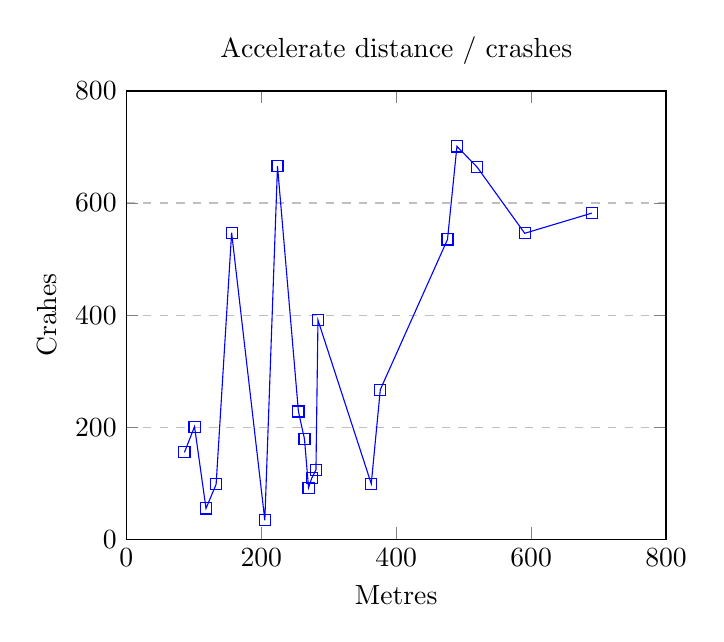
\begin{tikzpicture}
\begin{axis}[
    title={Accelerate distance / crashes},
    xlabel={Metres},
    ylabel={Crahes},
    xmin=0, xmax=800,
    ymin=0, ymax=800,
    legend pos=north west,
    ymajorgrids=true,
    grid style=dashed,
]

\addplot[
    color=blue,
    mark=square,
    ]
    coordinates{
    (86,155)(101,201)(118,55)(133,98)(156,547)(205.2,34)(224,666)(255,228)(264,179)(270,92)(274.7,109)(281,124)(284,391)(363,99)(376.4,267)(476,535)(490,701)(520,664)(590.5,546)(690,582)
    };
    %    \legend{CuSO$_4\cdot$5H$_2$O}

\end{axis}
\end{tikzpicture} \\

http://www.dictionary.com/browse/grand-prix
\end{document}

86, brake: 25 -- Monaco, crashes: 155
101, brake: 150 -- Belgium, crashes: 201
118, brake: 200 -- Austria, crashes: 55
133, brake: 125 -- Canada, crashes: 98
156, brake: 50 -- Azerbaijan, crashes: 547
205.2, brake: 0 -- Russia, crashes: 34
224, brake: 50 -- Singapore, crashes: 666
255, brake: 50 -- UAE, crashes: 228
264, brake: 100 -- USA, crashes: 179
270, brake: 0 -- Great Britain, crashes: 92
274.7, brake: 50 -- China, crashes: 109
281, brake: 100 -- Australia, crashes: 124
284, brake: 50 -- Brazil, crashes: 391
363, brake: 10 -- Japan, crashes: 99
376.4, brake: 100 -- Bahrain, crashes: 267
476, brake: 100 -- Hungary, crashes: 535
490, brake: 125 -- Italy, crashes: 701
520, brake: 100 -- Malaysia, crashes: 664
590.5, brake: 100 -- Spain, crashes: 546
690, brake: 200 -- Mexico, crashes: 582

